
\documentclass[12pt,a4paper,UTF8]{article}
\usepackage{ctex} % Chinese support
\usepackage{graphicx} % Insert images
\usepackage{listings} % Print source code
\usepackage[usenames,dvipsnames]{xcolor}
\usepackage{color} % Color support
\usepackage{float}
\usepackage{booktabs} % Professional table support
\usepackage{pdflscape} % Landscape pages support in PDF
\usepackage{hyperref} % Hypertext links support for cross-referencing
% \lstnewenvironment{cpp}{\lstset{language=cpp,
% 	basicstyle=\ttfamily\footnotesize,
% 	keywordstyle=\bfseries\color[rgb]{0, 0, 1},
% 	identifierstyle=\color[rgb]{0.5, 0.3, 0.1},
% 	stringstyle=\color[rgb]{0.6, 0.1, 0.1},
% 	commentstyle=\itshape\color[rgb]{0.05, 0.5, 0.05},
% 	backgroundcolor=\color[gray]{0.95},
% 	numbers=left,numbersep=5pt,numberstyle=\color[gray]{0.6},
% 	breaklines=true}}{}
\definecolor{mygreen}{rgb}{0,0.6,0}
\definecolor{mygray}{rgb}{0.5,0.5,0.5}
\definecolor{mymauve}{rgb}{0.58,0,0.82}
\lstset{
 backgroundcolor=\color{lightgray}, 
 basicstyle = \footnotesize,       
 breakatwhitespace = false,        
 breaklines = true,                 
 captionpos = b,                    
 commentstyle = \color{mygreen}\bfseries,
 extendedchars = false,             
 frame =shadowbox, 
 framerule=0.5pt,
 keepspaces=true,
 keywordstyle=\color{blue}\bfseries, % keyword style
 language = C++,                     % the language of code
 otherkeywords={string}, 
 numbers=left, 
 numbersep=5pt,
 numberstyle=\tiny\color{mygray},
 rulecolor=\color{black},         
 showspaces=false,  
 showstringspaces=false, 
 showtabs=false,    
 stepnumber=1,         
 stringstyle=\color{mymauve},        % string literal style
 tabsize=2,          
 title=\lstname                      
}

% Customize hyperref format (it's set to no special format here)
\hypersetup{hidelinks}

% Declare directories to search for graphics files for graphicx
\graphicspath{{figures/}{logo/}}


% Define source code style for listings
\lstdefinestyle{verilog}{
  language=Verilog,
  basicstyle=\ttfamily\footnotesize,
  keywordstyle=\bfseries\color[rgb]{0, 0, 1},
  identifierstyle=\color[rgb]{0.3, 0.2, 0},
  stringstyle=\color[rgb]{0.6, 0.1, 0.1},
  commentstyle=\itshape\color[rgb]{0.05, 0.5, 0.05},
  backgroundcolor=\color[gray]{0.98},
  numbers=left,
  numbersep=5pt,
  numberstyle=\color[gray]{0.6},
  breaklines=true
}

% Define source code style for listings
\lstdefinestyle{cpp-style}{
  language=C++,
  basicstyle=\ttfamily\footnotesize,
  keywordstyle=\bfseries\color[rgb]{0, 0, 1},
  identifierstyle=\color[rgb]{0.5, 0.3, 0.1},
  stringstyle=\color[rgb]{0.6, 0.1, 0.1},
  commentstyle=\itshape\color[rgb]{0.05, 0.5, 0.05},
  backgroundcolor=\color[gray]{0.95},
  numbers=left,
  numbersep=5pt,
  numberstyle=\color[gray]{0.6},
  breaklines=true
}

% Define new command for title page
\newcommand{\reporttitle}[2]{
  \LARGE\textsf{#1}\quad\underline{\makebox[12em]{#2}}
}
\newcommand{\reportinfo}[2]{
  \large\makebox[4em]{\textsf{#1}}\quad\underline{\makebox[18em]{#2}}
}
% The document begins here
\begin{document}
  \begin{titlepage}
    \centering
    
    
\includegraphics[height=144pt]{figure/picture.png}\\[48pt] % Change the school logo here (See the logo/ directory) and adjust the height
    {\huge\textsf{植\ 物\ 大\ 战\ 僵\ 尸}}\\[48pt]
    \reporttitle{报告名称}{PVZ设计}\\[72pt]

    \reportinfo{课程名称}{高级程序设计}\\[8pt]
    \reportinfo{学生姓名}{时欣}\\[10pt]
    \reportinfo{学\hspace{\fill}号}{191220097}\\[8pt]
    \reportinfo{实验日期}{2021年5月25日}\\
        \vspace*{\fill}
  \end{titlepage}

  \tableofcontents
  \newpage

  \section{实验内容}
    实现一个qt版的图形界面的植物大战僵尸,主要内容包括:
    \subsection{界面显示}
        \begin{enumerate}
          \item 5行9列的地块;
          \item 商店内容的显示;
          \item 阳光拥有值的显示
          \item 能够利用鼠标选择植物进行购买与种植
          \item 每个地块可以有多个僵尸
          \item 能够对游戏进行停止
          \item 有主界面和关卡选择
          \item 有bgm
          \item 能够用铲子去除植物
        \end{enumerate}

    \subsection{游戏主体}
        \begin{enumerate}
          \item 僵尸:普通僵尸,路障僵尸,读报僵尸,铁桶僵尸,铁网门僵尸, 撑杆僵尸,投石僵尸, 小丑僵尸;
          \item 植物:豌豆射手,双发射手,寒冰射手,坚果墙,土豆雷,樱桃炸弹,可以铲除植物的铲子;
          \item 攻击工具:普通子弹,寒冰射手的子弹,左侧的小推车;
        \end{enumerate}

    \subsection{游戏逻辑}
        \begin{enumerate}
          \item 塔防逻辑:植物有其对应的生命值和攻击力(每秒对僵尸造成多少伤害),僵尸有其对应的生命值,攻击力(每秒对植物造成多少伤害)和速度(走到
          下一个地块需要多少秒)。\\
                        当僵尸走到植物所在地块时可以对植物进行攻击;当植物的生命值减到0则植物死亡,从植物列表中移除,而僵尸可以走到下一个地
            块对其中的植物攻击。如果僵尸将最左侧地块的植物攻击致死,则游戏失败。\\
            其中对于植物
          \begin{enumerate}
            \item 豌豆射手、双发射手和寒冰射手的作用是每秒发射子弹,真正起作用的是子弹。子弹有其伤害值(一个子弹对僵尸造成多少伤害)和速度,当子弹与僵尸在同一个地块时,
            子弹对僵尸造成伤害,随后子弹消亡。当僵尸的生命值减到0则僵尸死亡。而寒冰射手的子弹还会让僵尸减速。
            \item 坚果墙、高坚果以及南瓜头没有攻击功能,只能在其还存活时对僵尸造成阻挡作用。
            \item 土豆雷的作用是当僵尸走到有它的地块,则使僵尸死亡并且自身死亡。
            \item 樱桃炸弹的作用是以自己为中心3*3范围内的僵尸死亡并且自身死亡。
            \item 大蒜在被攻击时将僵尸驱逐到临近行。
          \end{enumerate}
          而对于僵尸
          \begin{enumerate}
            \item 移动逻辑中,即所有僵尸都是能正常经过没有植物的地块,如果当前地块有植物那么必须要将其消灭才能继续前进。(投石僵尸和撑杆僵尸以下特别讨论)。
            \item 普通僵尸只有当所在地块有植物时对它进行攻击,撑杆僵尸也是。\\
                  路障僵尸、足球僵尸、铁桶僵尸、铁网门僵尸和普通僵尸的攻击逻辑相同,只是生命值更高。\\
                  读报僵尸和普通僵尸的攻击逻辑相同,只是受到攻击后速度会加快。\\
                  投石僵尸在有石头的时候用石头对植物攻击。没有石头直接前进并且碾压植物。
          \end{enumerate}

          \item 购买逻辑:植物有其对应的阳光消耗值,选定购买以后,阳光拥有值扣除相应的数量。如果阳光拥有值不足,则无法购买。如果冷却时间不够,则无法购买。冷却时间
          需要用矩形块显示。
          \item 种植逻辑:如果当前地块没有种植植物则可以种植。否则不能种植。
          
        \end{enumerate}
    

\section{实验目标}
    实现较好的交互界面,完成游戏正确的逻辑,丰富植物和僵尸的种类。

\section{实验环境}
\begin{enumerate}
  \item 设计语言:c++
  \item 运行环境:Windows
  \item 设计环境:qt
\end{enumerate}
  
\section{相比较第二阶段的变动}
每一个植物有自己的冷却时间,而不是全部共享一个冷却时间
增加暂停功能,音乐,小推车,以及图形界面,僵尸种类等等

\section{实验设计思路}
    运用c++语言,运用面向对象的思路设计。
    \begin{enumerate}
      \item 需要实现的各类间关系如下图
          \begin{figure}[H]
            \centering
          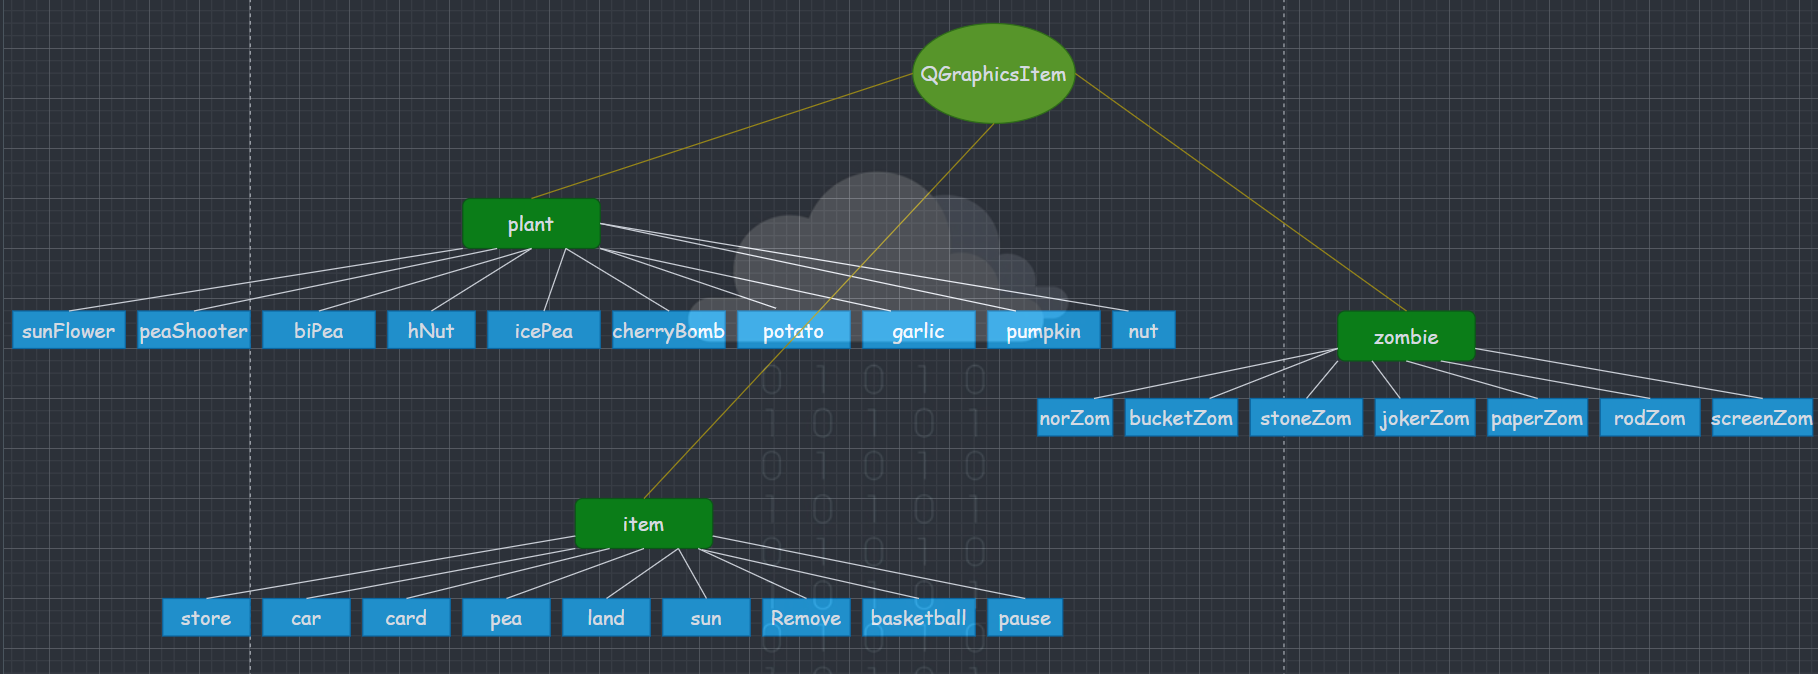
\includegraphics[width=0.9\textwidth]{figure/UMI.png}
          \caption{各类间关系}
          \end{figure}
    \item 设计思路\\
          本次的实验采用了Graphics View框架。它实现了模型-视图结构的图形管理,能对大量图元进行管理,支持碰撞检测,坐标变换和图元组等多种方便的功能。\\
          GraphicsView框架结构主要包含三个主要的类QGraphicsScene(场景)、QGraphicsView(视图)、QGraphicsItem(图元)。QGraphicsScene本身不可见,是一个存储图元
          的容器,必须通过与之相连的QGraphicsView视图来显示及与外界进行交互,主要提供图元的操作接口、传递事件和管理各个图元状态,提供无变换的绘制功能(如打印);
          QGraphicsView提供一个可视的窗口,用于显示场景中的图元,一个场景中可以有多个视图。QGraphicsItem是场景中各个图元的基础类,QT提供了常用图形图元的标准类,
          如矩形(QGraphicsRectItem)、文本(QGraphicsTextItem)。\\

          而上图正是给出了继承自QGraphicsItem的类及它们子类间的关系。\\

          即QGraphicsItem的派生类是游戏场景中的各个游戏主体。\\

          关于主场景(开始界面)和游戏关卡的切换,采用了信号槽机制,即通过将鼠标点击发出的信号通过connect函数处理。实现的效果为点击“fight1”按钮跳转至
          游戏界面并且游戏开始。

    \end{enumerate}

\section{各个类的设计}
    \subsection{zombie类}
      \begin{figure}[H]
        \centering
      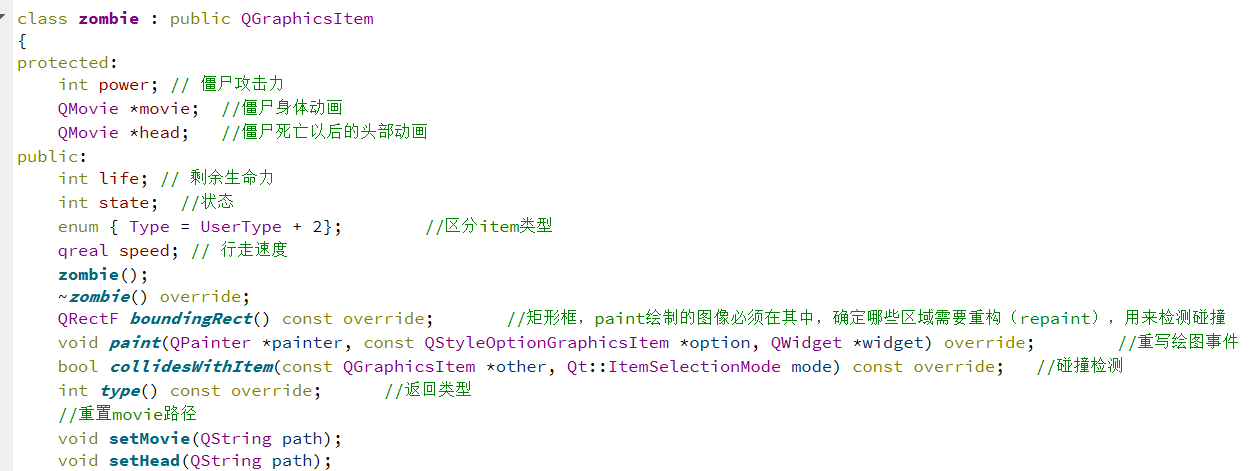
\includegraphics[width=0.7\textwidth]{figure/zombie.png}
      \caption{zombie类数据与操作}
      \end{figure}
      各个数据成员与成员函数的含义如注释所标。作为QGraphicsItem的子类,重写boundingRect,paint和collidesWithItem函数时有必要的,需要对碰撞进行检测并作出合适的逻辑处理,
      而paint中需要对僵尸被减速时的gif作标蓝处理。

      \subsubsection{普通僵尸}
        其实非常简单,只需要写构造函数和重写advance函数。
        构造函数就是对僵尸的各种值进行设置,而advance函数则是在僵尸状态发生变化的时候,对其的显示作出变化,分为从行走到攻击,从攻击到行走,以及从或者到死亡,以及死亡gif播放结束
        这四种情况。并且僵尸的攻击逻辑也在advance函数中实现,即通过collidingItems()查看是否有与之碰撞的植物,如果有则对植物进行攻击,植物生命值减少相应的伤害值。
        \begin{figure}[H]
          \centering
        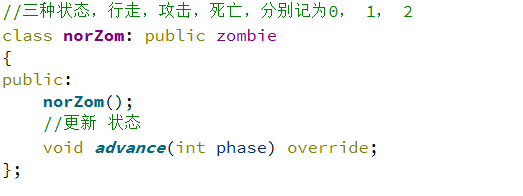
\includegraphics[width=0.6\textwidth]{figure/norZom.png}
        \caption{norZom类数据与操作}
        \end{figure}
        而除了读报僵尸以外的其他僵尸,以上逻辑和普通僵尸完全一样,只是数值略有不同,因此不做赘述。
      \subsubsection{读报僵尸}
        同样是对这两个函数进行实现。然而由于读报僵尸的特殊性,在其报纸被打掉(实际实现时,就是生命值降到满值的一半时算作报纸的防御消失),此时需要将其的动画改成
        无报纸的形式,并且将其加速,而且加速只能一次。因此比以上的0,1,2多了两种状态。截取部分如下图
        \begin{figure}[H]
          \centering
        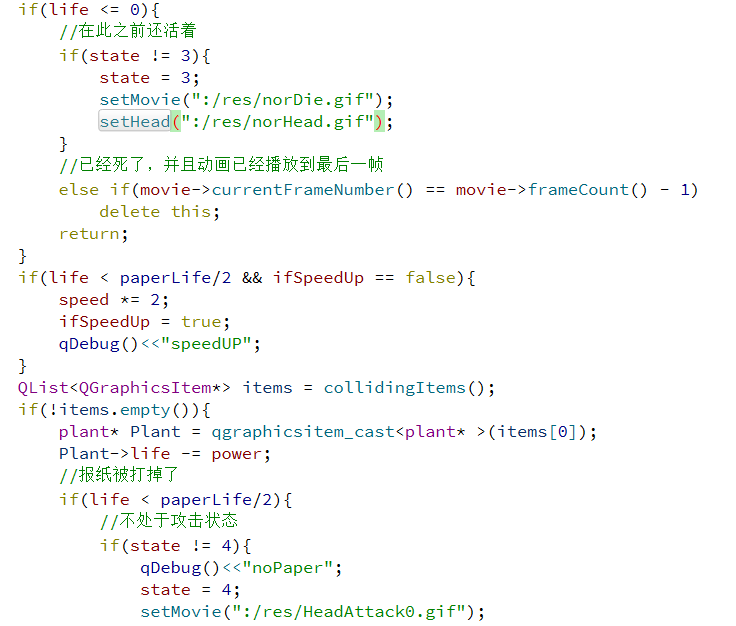
\includegraphics[width=0.6\textwidth]{figure/paperZom1.png}
        \caption{paperZom类数据与操作}
        \end{figure}

    \subsubsection{撑杆僵尸}
        \begin{figure}[H]
          \centering
        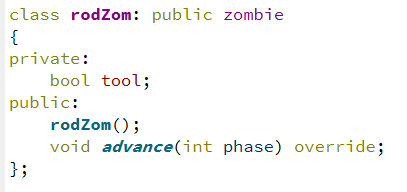
\includegraphics[width=0.6\textwidth]{figure/rodZom.png}
        \caption{rodZom类数据与操作}
        \end{figure}
        和上面的实现差不多,只是移动逻辑有一些变化,为此增加了tool来表示是否还有杆子。在advance中如果检测到与植物碰撞并且有杆子,那么切换为jump状态,当发现jump的gif到最后一帧的时候
        则切换为无杆状态。但是会判断有杆时有与其碰撞的植物是否是高坚果,如果是的话就不能跳跃只能攻击。而死亡的状态逻辑和上述僵尸一样,不再赘述。

    \subsubsection{投石僵尸}
      \begin{figure}[H]
        \centering
      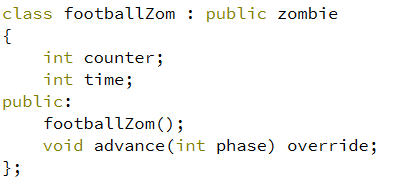
\includegraphics[width=0.6\textwidth]{figure/stoneZom.png}
      \caption{stoneZom类数据与操作}
      \end{figure}
      (因为实在找不到投石僵尸的资源,所以僵尸的gif用足球僵尸替代了,并且拿了一张篮球的图片当攻击工具。)\\
      依旧是构造函数和advance。此处增加了两个数据成员,即counter和time。用来定时发射篮球攻击植物。由于在框架之中我并没有记录每个植物、僵尸的坐标、所以当时实现它的攻击逻辑的时候
      出现了一点小问题————即如何判断这一行上有植物。毕竟之前的攻击都是通过collidesWithItem实现的。而现在需要在和植物碰撞之前就知道这一行到底有没有植物。因此我选择了在store这个类
      里面增加了一个成员,即plantNum。这是一个有五个元素的数组,用来记录每一行有几个植物。它的改动发生在两个时刻————种植植物的时候,对应的那一行计数+1;植物死亡的时候,对应的那一行
      计数-1。因此每次投石僵尸出现的时候,它会首先判断还有没有石头,如果还有石头那么就会判断这一行有没有植物(访问store的计数数组),如果有植物则投放石头;如果没有则直接前进。如果没有
      石头那么直接前进,并且压死路上的所有植物。所以要做的有几个动作————1)life<=0则播放死亡动画;2)如果满足投放石头的条件投放石头,而石头也即篮球的逻辑由生成的篮球自行完成;
      3)满足前进条件则前进。(对于坐标的确定是通过对x()和y()的处理得到的)。\\
      注意它的攻击在有南瓜头的情况下,是攻击南瓜头保护的那个植物。如果只有南瓜头才是攻击南瓜头。

    \subsubsection{小丑僵尸}
    \begin{figure}[H]
      \centering
    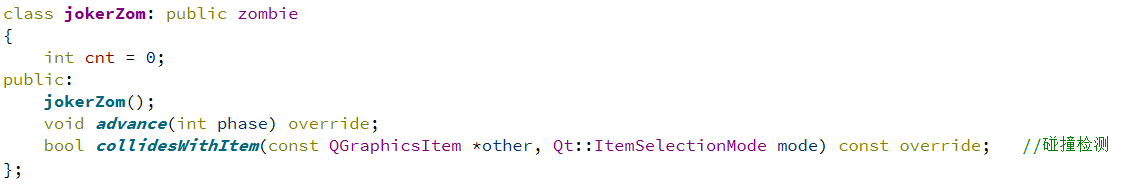
\includegraphics[width=0.6\textwidth]{figure/jokerZom.png}
    \caption{stoneZom类数据与操作}
    \end{figure}
    小丑僵尸的碰撞需要注意它的碰撞检测得根据所处的状态不同,即当其在正常状态下只会攻击所在地块上的植物,而当其爆炸时会炸毁其周围的植物。\\
    而关于advance,我设置了cnt实现定时生成随机数来决定小丑僵尸要不要爆炸。如果要爆炸则遍历与其碰撞的植物将其delete。否则则和普通僵尸的逻辑相同。

    \subsubsection{与南瓜头、大蒜的攻击逻辑}
    这些僵尸有个共性,就是在攻击植物的时候。如果一个地块有两个植物(其中一个是南瓜头),那么僵尸会优先攻击非南瓜头的那个植物(不包括投石僵尸)。而如果攻击了大蒜,那么僵尸会随机到
    相邻行,也即需要改变它的位置。通过判断plant的t来帮助实现。

       
    \subsection{plant类}
      \begin{figure}[H]
        \centering
      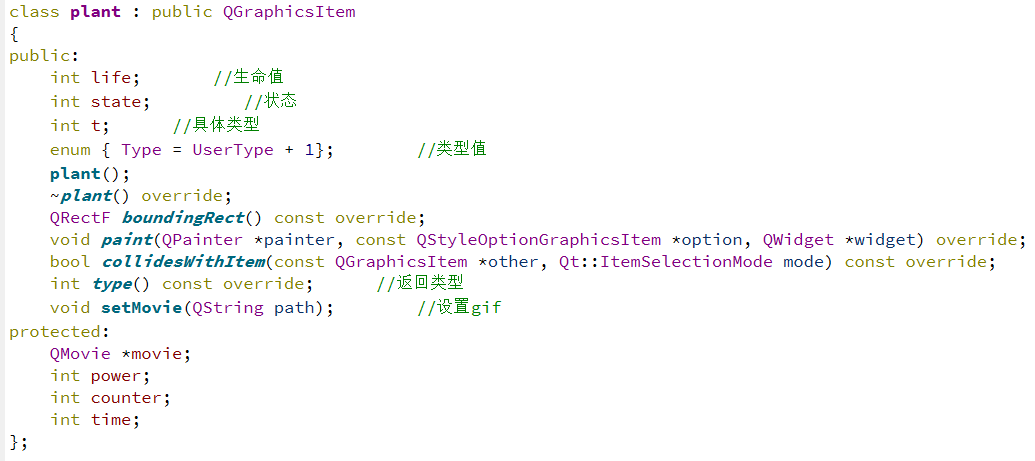
\includegraphics[width=0.65\textwidth]{figure/plant.png}
      \caption{plant类数据与操作}
      \end{figure}
      各个数据成员与成员函数的含义如注释所标,其中的t是为了区分不同的植物,以备后续的攻击逻辑。其中需要重写的函数其实与僵尸类似,不作赘述,下面展示各个具体植物的实现。

    \subsubsection{peaShooter类}
    \begin{figure}[H]
      \centering
    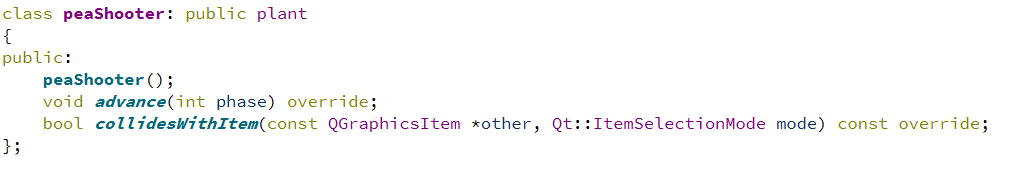
\includegraphics[width=0.6\textwidth]{figure/peaShooter.png}
    \caption{peaShooter类数据与操作}
    \end{figure}
    重写了advance和collidesWithItem函数。advance用于定时在场景上添加子弹,而collidesWithItem依旧是检测碰撞。
    \subsubsection{potato类}
      \begin{figure}[H]
        \centering
      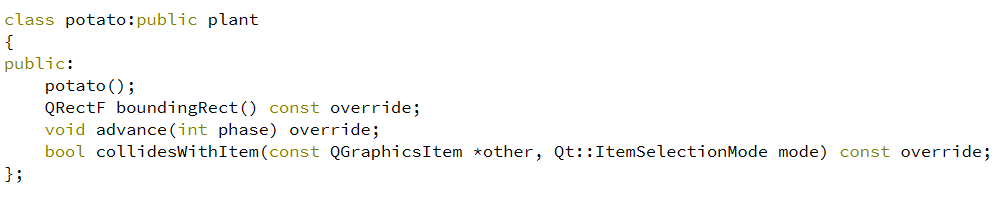
\includegraphics[width=0.6\textwidth]{figure/potato.png}
      \caption{potato类数据与操作}
      \end{figure}
      依旧需要重写advance和collidesWithItem函数,此外还包括boundingRect,因为土豆雷根据其状态不同会需要重新绘制。
      相比较peaShooter,它会稍微再复杂一点。我设置了一个counter用来计数,在第一次到达time的时候进入攻击状态,第二次到达time的时候发动攻击,炸毁与它碰撞的
      僵尸,并且放映自身的爆炸动画,并将僵尸从scene上移除
    \subsubsection{sunFlower类}
      其成员函数和peaShooter相同,且advance逻辑也相同,只是把peashooter的定时添加子弹,变成了定时添加阳光。
    \subsubsection{icePea类}
      其实现与peashooter一模一样,只是生成的子弹类型为1,表示是可以减速的子弹
    \subsubsection{biPea类}
    其实现与peashooter一模一样,只是生成的子弹速度设置为peashooter的两倍
    \subsubsection{cherrybomb类}
      其实现的函数与逻辑和potato类一模一样,只是advance类里面会在炸死在它炸毁范围内的僵尸的时候,播放僵尸的炸毁动画。
    \subsubsection{nut类、hNut类、pumpkin类,garlic类}
      成员函数仅包括构造函数和advance函数。在advance函数中会根据其生命值的大小改变其放映的gif效果。非常简单

    \subsection{item类}
    \begin{figure}[H]
      \centering
    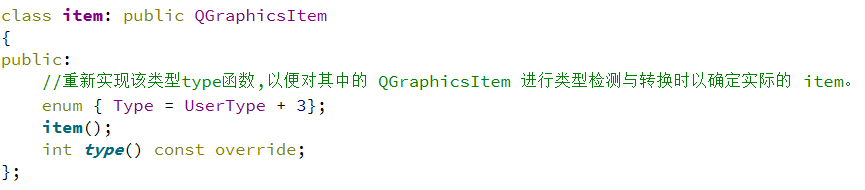
\includegraphics[width=0.7\textwidth]{figure/item.png}
    \end{figure}
    这个类的派生类属于游戏主体中除了僵尸和植物以外的东西,基类中的成员非常简单,仅包含类型属性和构造函数。主要在于其派生类的具体实现:
    \subsubsection{car类}
    \begin{figure}[H]
      \centering
    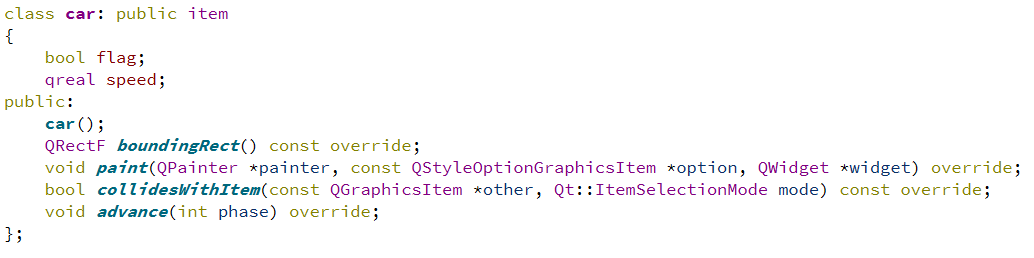
\includegraphics[width=0.7\textwidth]{figure/car.png}
    \end{figure}
    这个类实现的是草坪左侧的小推车。其攻击逻辑包括在advance函数里,即只有在其范围内出现了僵尸,它才会开始移动,并且将这一排的僵尸全都压死。为此设置了一个
    标志位flag,一旦flag被设置为1,则车不断的移动,直到走到界面以外
    \begin{figure}[H]
      \centering
    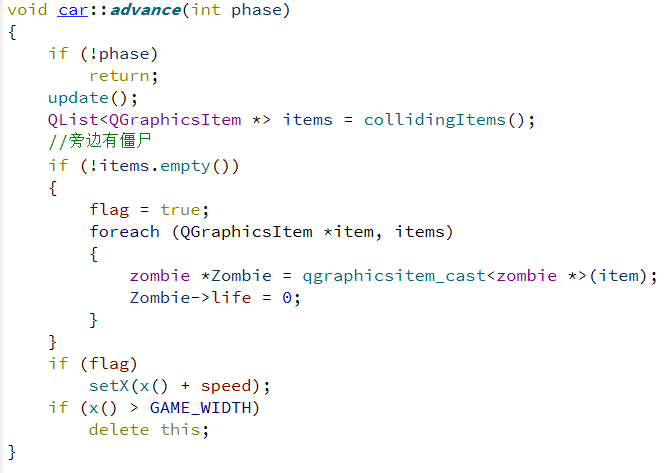
\includegraphics[width=0.7\textwidth]{figure/carAdvance.png}
    \end{figure}

    \subsubsection{card类}
    \begin{figure}[H]
      \centering
    
\includegraphics[width=0.7\textwidth]{figure/card.png}
    \end{figure}
    各个成员函数和数据成员函数如图所标。注意卡片会被点击,需要接受点击事件并且对其作出处理,所以需要重写关于mouse的一系列事件
    \begin{figure}[H]
      \centering
    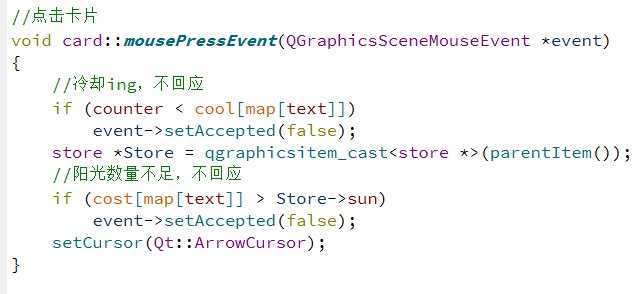
\includegraphics[width=0.7\textwidth]{figure/mousepress.png}
    \end{figure}
    注意在接收事件之前需要判断阳关数量是否充足以及冷却时间是否结束,从而判断是否要接受这个点击事件
    \begin{figure}[H]
      \centering
    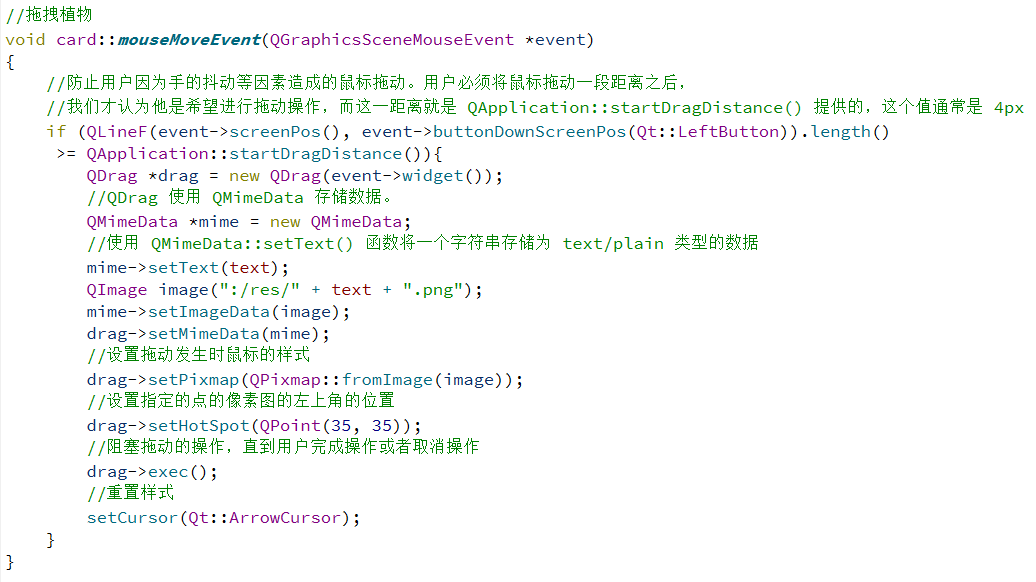
\includegraphics[width=0.7\textwidth]{figure/mousemove.png}
    \end{figure}
    首先我们利用QLineF得到拖拽的距离是否超过一定的值,避免用户是因为手抖的选择,然后做出一系列处理(含义如图片所标注)。\\
    然后重载mouseReleaseEvent函数,即设置一下鼠标的样式。\\
    而对于冷却时卡片的动画效果,采用了brush来绘制。
    \begin{figure}[H]
      \centering
    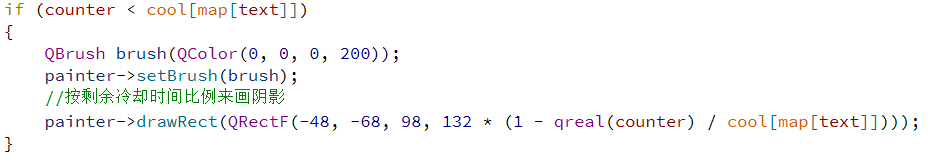
\includegraphics[width=0.7\textwidth]{figure/brush.png}
    \end{figure}

    \subsubsection{land类}
    这个类是有关种植植物的逻辑
    \begin{figure}[H]
      \centering
    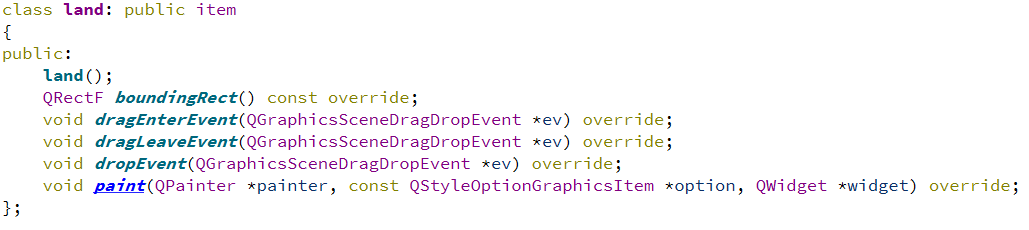
\includegraphics[width=0.7\textwidth]{figure/land.png}
    \end{figure}
    注意到需要重写dragEnterEvent,dragLeaveEvent,dropEvent函数,来使得在点击卡片并且松手以后能够实现植物的种植————即在场景上的显示
    \begin{figure}[H]
      \centering
    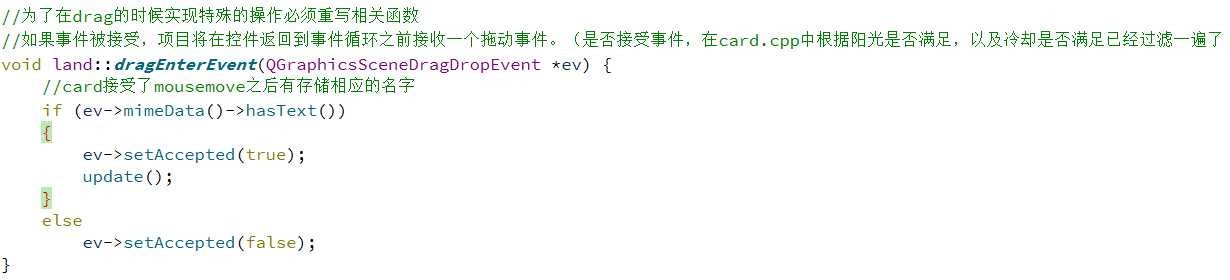
\includegraphics[width=0.7\textwidth]{figure/dragenter.png}
    \end{figure}
    可以看到在dragenter函数当中,根据QDrag的存储结构QMimeData是否标上了名字来确认之前的鼠标事件是否有效。\\
    而在dropEvent函数中,需要根据鼠标被放下的位置转换成scene的坐标,然后调整系数来将item放到正确的位置。而这里需要注意,即点击的可能是卡片,也可能是铲子,所以需要进行判断。
    如果是卡片则在对应位置增加植物,而如果是铲子,那么需要将对应地块存在的植物铲除。
    重载paint是发现不加这个会通不过编译,但其实paint并没有什么事件。

    \subsubsection{pause类}
    这个类与游戏的暂停键相关。
    \begin{figure}[H]
      \centering
    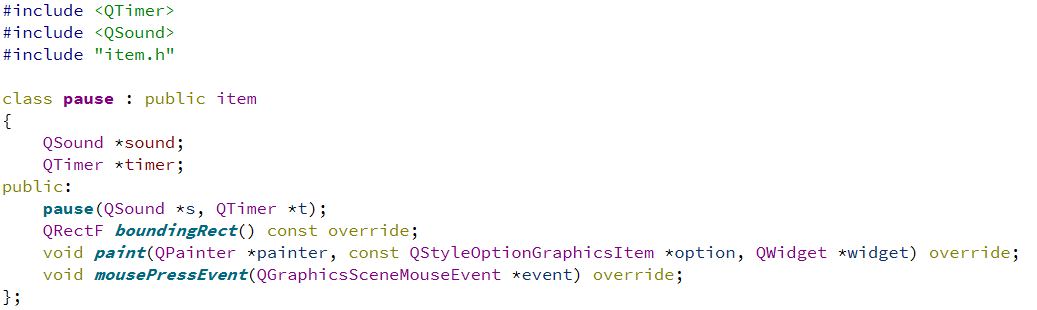
\includegraphics[width=0.7\textwidth]{figure/pause.png}
    \end{figure}
    它有两个数据成员,即构造时会传入游戏的计时器以及背景音乐的变量。\\
    重写绘画事件比较简单,但是需要注意,要根据timer的开启(暂停)情况,在按钮上写不同的文字。\\
    press事件也非常简单,当左键点击暂停键以后————如果计时器活跃,那么将其暂停,并且音乐暂停。否则,继续游戏和音乐。

    \subsubsection{remove类}
    这个类与铲子有关
    \begin{figure}[H]
      \centering
    
\includegraphics[width=0.7\textwidth]{figure/remove.png}
    \end{figure}
    可以看到同样的需要重载boundingRect和paint事件,这两个比较简单不再详述。
    而mouseMoveEvent实际上还是和card那里拖拽卡片的处理是一样的,用QMimeData存储drag的相关信息,并且设置一系列相关显示即可。\\
    此处我们添加了函数removePlant,其实现为找到对应位置的item,并且对其进行删除。

    \subsubsection{store类}
    这个类与卡片商店有关
    同样的需要重载boundingRect和paint事件。除此以外我增加了sun成员,用来记录当前阳光数量。而定时增加阳光的逻辑正是在advance中实现的,当计数器counter自增到了规定好的time值,则
    阳光会增加25,并且在场景上增加sun这个item。\\
    函数addPlant用来在场景上根据传入的植物名字和位置添加植物,注意如果已经有植物了,那么直接返回不种植。否则,对应的阳光减去花费,并且新建对应的植物种在对应的植物。需要注意卡片的
    冷却计数需要从0开始。
    \begin{figure}[H]
      \centering
    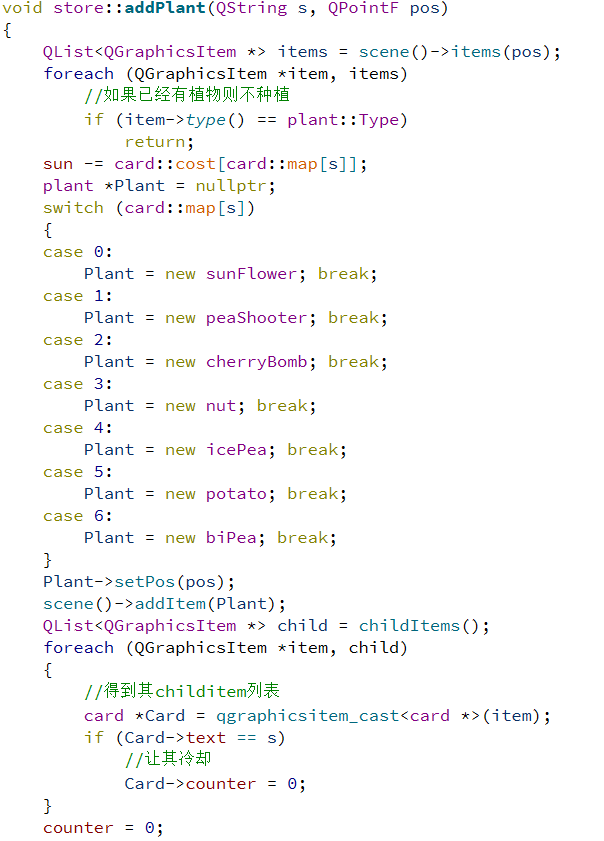
\includegraphics[width=0.7\textwidth]{figure/addPlant.png}
    \end{figure}

    \subsubsection{sun类}
    这个类对应阳光
    \begin{figure}[H]
      \centering
    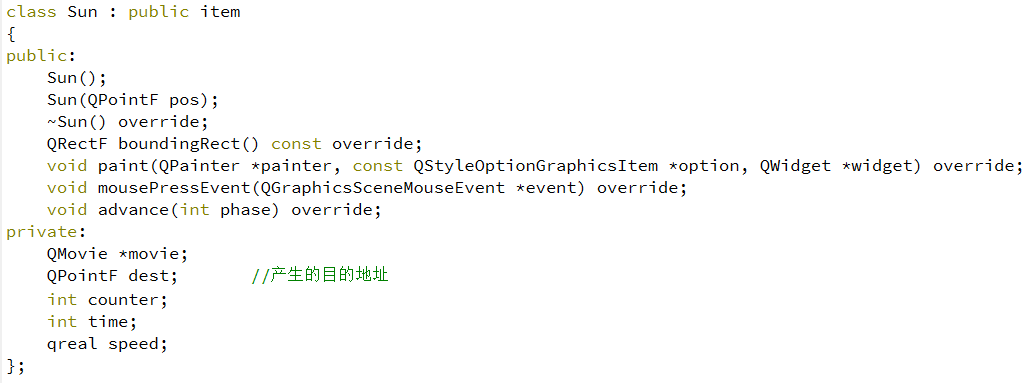
\includegraphics[width=0.7\textwidth]{figure/sun.png}
    \end{figure}
    我实现了两种构造函数,一种默认一种带参数的。默认的是为了系统产生阳光的时候,而带参数的是针对向日葵产生的阳光的。movie存储太阳的动画,dest存储阳光产生的目的地址,counter和time
    用来控制阳光的生存周期,speed控制阳光下落的速度。\\
    mousepress则是在阳光被点击的时候,将阳光的数值增加25。advance实现阳光的定时移动,并且在超时的时候删除阳光。

    \subsection{mainScene类}
    实现的是游戏的主场景,即开始界面。有一个选项“fight1”,点击后可以进入第一关。
    \begin{figure}[H]
      \centering
    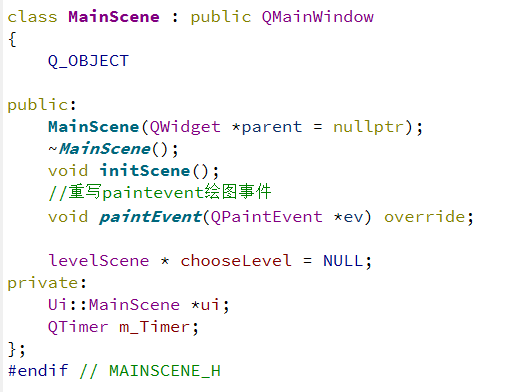
\includegraphics[width=0.7\textwidth]{figure/mainScene.png}
    \end{figure}
    这几个成员函数中最主要的是initScene和paint。添加的成员有timer,负责游戏的一些定时逻辑;有chooseLevel,对应的是具体关卡。\\
      在initScene中,有对窗口的初始化,设定窗口的名字和图标以及大小。
      \begin{figure}[H]
        \centering
      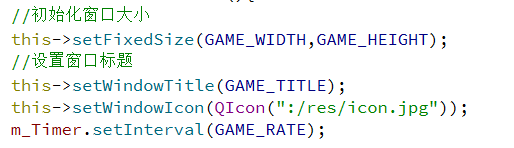
\includegraphics[width=0.7\textwidth]{figure/window.png}
      \end{figure}
      随后是对关卡选择按钮的设置
      \begin{figure}[H]
        \centering
      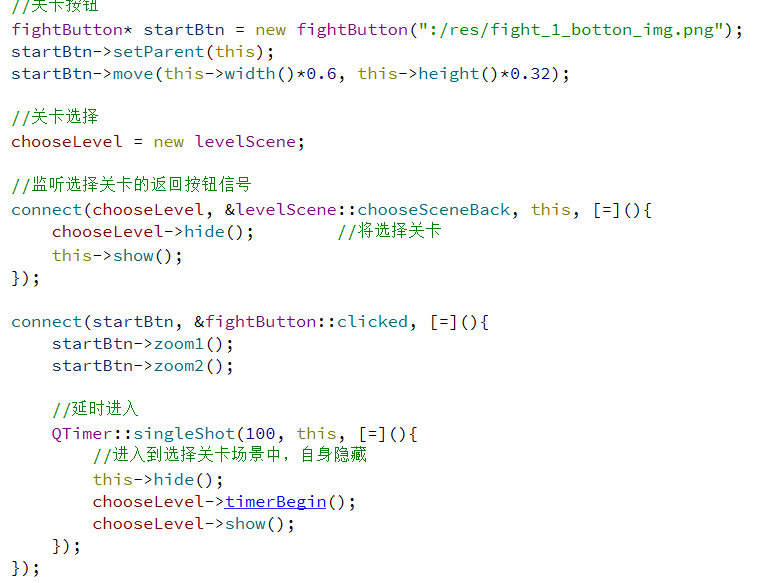
\includegraphics[width=0.7\textwidth]{figure/fightButton.png}
      \end{figure}
      通过qt的信息槽机制,用connect使得按钮被点击时做出相应动作。其中zoom1和zoom2是为了实现按钮被点击后的跳动效果,而被点击以后levelScene的计时器才会开始攻击。\\
      而paintEvent是为了绘制主界面背景。

    \subsection{levelScene类}
    \begin{figure}[H]
      \centering
    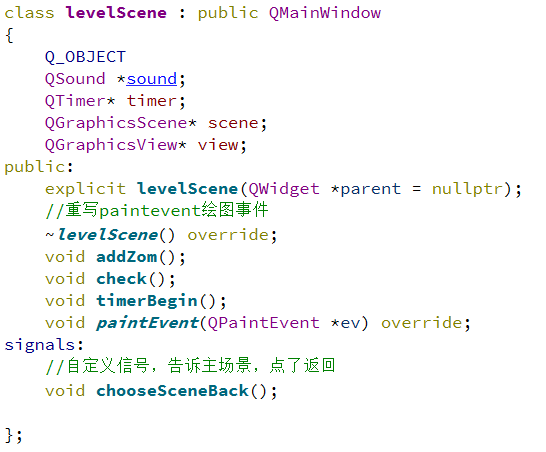
\includegraphics[width=0.7\textwidth]{figure/levelScene.png}
    \end{figure}
    私有成员增加了sound即背景音乐,timer即计时器,而scene和view是有关场景显示。\\
    \subsubsection{构造函数}
    构造函数里对一系列成员进行了初始化,包括设置场景标题、图标、大小;设置音乐开始播放;设置定时器;将scene绑定到当前类,并设置场景范围;设置暂停按钮;设置商店;设置land用于drag事件
    处理;设置小推车;设置场景背景并且显示。
    \subsubsection{timerBegin}
    设置计时器开始并且将定时器和check、addZom、advance绑定,实现定时调用的逻辑。
    \subsubsection{addZom}
    通过counter和time计数实现定时生成僵尸,并且根据随机数决定生成哪一种僵尸。
    \subsubsection{check函数}
    通过counter和time计数实现定时检查是否输掉,即发现僵尸的坐标已经到了范围以外进入了“家”里。

    \subsection{fightButton类}
    \begin{figure}[H]
      \centering
    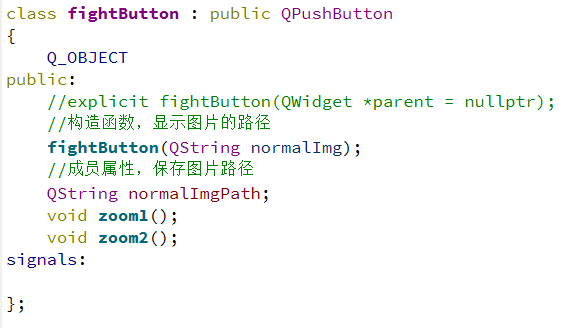
\includegraphics[width=0.7\textwidth]{figure/button.png}
    \end{figure}
    自己实现一个按钮类主要是为了按钮被点击时的上下晃动效果,也即以上的zoom1和zoom2。其实现以及代码注释如下。
    \begin{figure}[H]
      \centering
    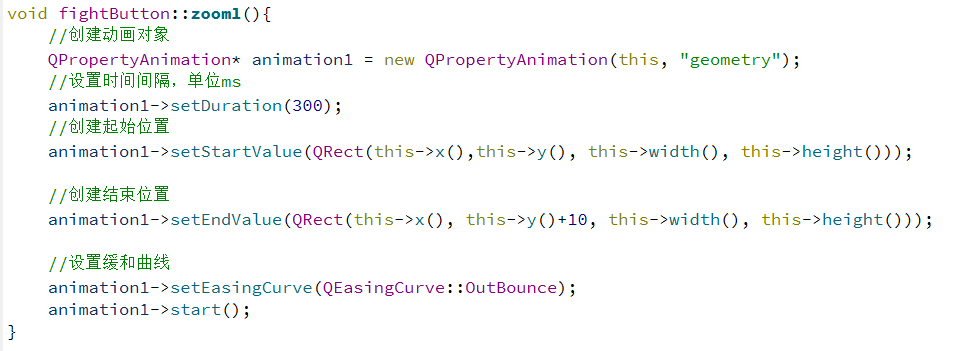
\includegraphics[width=0.7\textwidth]{figure/zoom.png}
    \end{figure}
  
    
\section{程序亮点}
\begin{enumerate}
  \item 选择了Graphics View框架和信号槽机制,框架逻辑清晰,对各个游戏主体进行了合理的组织。效果是使得整个游戏场景都非常尊重原版,包括gif、选择植物种植等等,几乎与原版一模一样。
  \item 游戏有主界面,有一个选项能够点击进入游戏场景,并且有晃动动画,在晃动以后延时一小会进入游戏场景。晃动动画比较好看。如下图
  \begin{figure}[H]
    \centering
  
\includegraphics[width=0.7\textwidth]{figure/start.png}
  \caption{主界面}
  \end{figure}
  \item 点击按钮则进入游戏界面,如下图。植物和僵尸都是gif实现。并且选择植物卡片拖拽的时候,鼠标拖动位置会显示对应植物的图片。对于避免用户手抖造成的鼠标事件有进行判断。卡片冷却的时候会
  有阴影的递减显示冷却时间剩余。僵尸被寒冰射手的子弹攻击到时会有蓝色被冰冻的效果。
  \begin{figure}[H]
    \centering
  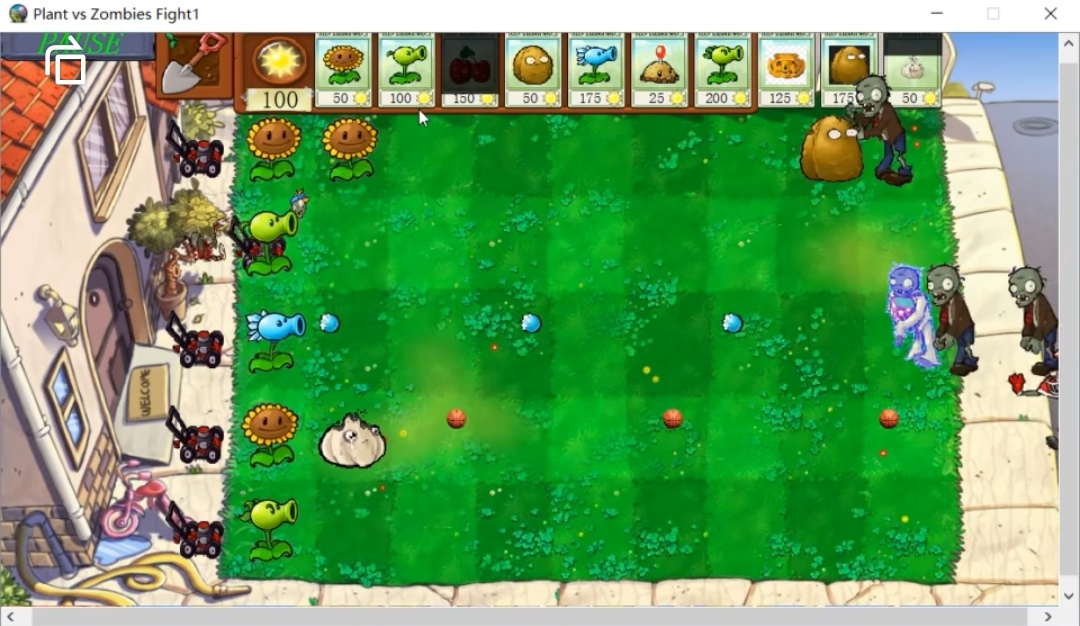
\includegraphics[width=0.7\textwidth]{figure/game.jpg}
  \caption{游戏界面}
\end{figure}
\end{enumerate}
 
\section{附加功能}
\begin{enumerate}
  \item 增加了铁网门僵尸和铁桶僵尸;
  \item 增加了铲子来铲除植物;
  \item 增加了小推车实现了和原版一样的一次拯救一下这一行的功能;
  \item 增加了暂停按钮可以使游戏暂停;
  \item 增加了主场景和具体关卡场景的切换;
  \item 增加了背景音乐。
\end{enumerate}
  
\section{玩法}
  \subsection{游戏开始界面}
  \begin{enumerate}
    \item 点击fight1按钮则进入游戏场景
  \end{enumerate}
  
  \subsection{商店购买规则}
  \begin{enumerate}
      \item 玩家可以通过点击对应的卡片来选择要种植的植物,并且进行拖拽,当拖拽事件结束,对应的植物会被种在松开鼠标所在的地块,而阳光总数减去对应的阳光消耗。但是当植物冷却时
      间未结束(即还有阴影被绘制在卡片上)以及阳光数量不够的时候,游戏不对此作出回应。注意一个地块不能种两个植物,除非有一个是南瓜头。
      \item 点击左上方的pause按钮可以对游戏进行暂停。暂停后按钮会变成“continue”,再次点击则游戏恢复进度。
      \item 点击左上方的小铲子并且放在对应的地块的时候可以将地块上的植物进行铲除。但是如果所在地块上没有植物那么没有反应。
  \end{enumerate}

  \subsection{攻击规则}
  \begin{enumerate}
    \item 一共有3行7列地块。僵尸会随机出现在某一行的最右侧地块。玩家需购买植物来守卫自己的家(在游戏界面的最左边)。购买货币为阳光,由系统定时生成已经可以购买向日葵来生成阳光,
    总数显示在商店的阳光图片下方。
    \item 现有植物为三种射手,其功能为定时产生子弹。当子弹打到僵尸时,对僵尸造成定量伤害,随后这颗子弹被消耗。樱桃炸弹可以炸毁周围3*3的僵尸。高坚果、坚果墙和南瓜头不能发动攻击但是
    可以防御抵挡。土豆雷可以将走到它旁边的僵尸炸毁。向日葵可以定时产生阳光。大蒜在收到攻击的时候将攻击它的僵尸驱逐到相邻行。\\
    如果僵尸走到植物所在的地块,那么僵尸可以对植物进行攻击,直到植物被僵尸伤害至生命值为0,僵尸才可以走到下一个地块。例外的是撑杆僵尸可以有一次跳过非高坚果的植物的机会。而投石僵尸
    可以有五次远程攻击本行植物的机会,用完篮球或者本行没有植物的时候可以前进。
    \item 如果僵尸走到了最左边的地块(即家所在的最后一道防线),且地块上的植物被攻击致死,那么僵尸到达了“家”,玩家游戏失败。
  \end{enumerate}

\section{遇到的问题以及解决方法}
\begin{enumerate}
  \item 其实遇到的问题倒是和逻辑实现没关系,主要是不熟悉qt的用法,进行搜索以后就解决了。
  \item 遇到了写了一个控件但是不显示的情况,结果发现是没有让它show。
  \item 以及写了mouse相关的事件,但是点击卡片发现没有反应,随后发现还要重写drag事件。
  \item 一开始在场景中添加植物的时候,是随便设置的位置,然后出大问题,所以增加了一些调试信息,找到了参考位置的坐标,然后进行运算找到植物的位置。
  \item 僵尸一开始实现的是定时产生僵尸,但是后来觉得后期应该快一点。但是改了以后发现快的没法控制,所以又增加了一些限制,
  \begin{figure}[H]
    \centering
  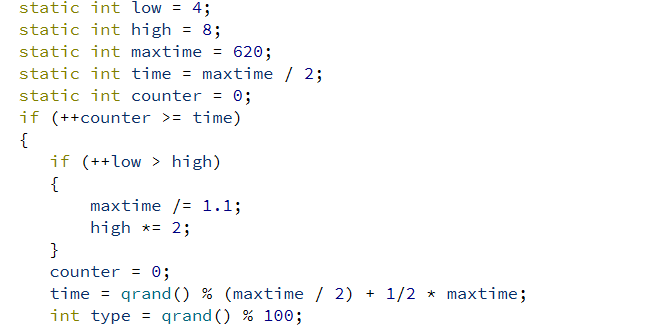
\includegraphics[width=0.7\textwidth]{figure/time.png}
  \end{figure}  
  即maxTime定时减少以及根据随机数减少,但是不会减少的太多。偶尔会骤降。
\end{enumerate}

\section{与前两次课设的关系}
\begin{enumerate}
  \item 游戏整体的逻辑还是不变的,只是实现因为所有的API不同发生了变化。比如原来是判断坐标是不是在一起,需要进行坐标判断。而现在可以直接用qt提供的函数即collidesWithItem就可以判断与其
  碰撞的item进行攻击逻辑。
  \item 并且也不再需要while循环里面一个一个调用函数,还需要计数定时增加阳光等等。而是可以使得对应场景设置定时器,通过信号来让函数定时被调用。
  \item 也因此,购买植物不再需要停止其它逻辑去处理,而是可以直接利用qt提供的功能即鼠标事件等相关的函数,实现购买和其他逻辑的同步。
  \item 继承依然在被使用,并且派生类对一些函数进行重载,从而实现动态绑定来调用具体的不同item对应的函数。
\end{enumerate}



\section{总结与感想}
因为以前不会qt,所以一开始真的非常非常痛苦。而且又有ddl压着,总觉得来不及。跟着教程学qt以及看了一些样例,慢慢地上手才来了感觉,逐渐知道怎么写。学习一个软件最好的方法还是得动手,光看
教程基本没什么用。期间有bug一直de不出来的情况,qt的GraghicsView类中坐标真的很重要,因为需要用坐标去访问,触发很多事件,一旦坐标没有写对,那么对应的逻辑必然无法实现,呈现出什么都没有
的效果。另外的很多的事件逻辑由一个完整的过程,比如先设置其参数、状态,然后需要将其加入什么里面或者绑定到什么里面,又或者让其开始执行or显示,它才能实现正确的逻辑。写代码的时候应该时刻
清楚自己已经做了哪些工作,还有哪些没有完成,才能实现整个完整正确的逻辑。\\
通过这次实验我成功写了小时候一直玩的游戏,说实话根本没想到自己能写出来,并且最终的效果同学们都说很像原版,还是很高兴的。还顺带着学习了qt的使用方法。\\
最后,感谢老师和学长们的辛苦付出!



%\lstinputlisting[style=verilog]{md5_inout.v}

      
  \end{document}



